\documentclass[a4paper,12pt]{article}
\usepackage{graphicx}
\usepackage{bm,amssymb}
\usepackage{mathrsfs}
\usepackage[unicode,colorlinks=true,filecolor=blue, menucolor=black, linkcolor=black, citecolor=black,pagebackref=white]{hyperref}
\usepackage[utf8]{inputenc}
\usepackage[russian]{babel}
\usepackage{amsmath}
\usepackage{feynmp}
\usepackage{caption}
\usepackage[left=2cm,right=2cm, top=2cm,bottom=2cm,bindingoffset=0cm]{geometry}
\begin{document}

\section{Трансцендентные уравнения}

\subsection{Вступление}

В приложениях очень часто приходится иметь дело с трансцедентными
уравнениями, зависящими от одного или нескольких параметров. Как правило,
они не имеют аналитического решения, а только численное; однако наличие
в таких задачах малого или большого параметра на практике помогает
найти приближённый вид ответа.


\subsection{Задача 1 (намагниченность ферромагнетика в теории среднего поля)}

Решим уравнение 
\[
m=\tanh(m/T)
\]


\noindent
Оно всегда имеет тривиальное решение $m=0$; однако, существует критическая
точка $T=T_{c}$, вблизи которой появляется нетривиальное решение
$m(T)$. Найти асимптотическое поведение этого решения вблизи критической
точки (при $\left|T-T_{c}\right|\ll T_{c}$), а также вблизи нуля
(при $T\ll T_{c}$).


\subsubsection{Решение}

Решать задачу будем графически. Для удобства сделаем перемасштабирование
- введем $\tilde{m}=m/T$; уравнение перепишется как $T\tilde{m}=\tanh\tilde{m}$.
Нарисуем на графике левую и правую часть уравнения.

\begin{figure}[h]
	\caption{$T\tilde{m}=\tanh(\tilde{m})$, $T=3;\,1;\,0.5$}
	\centering
	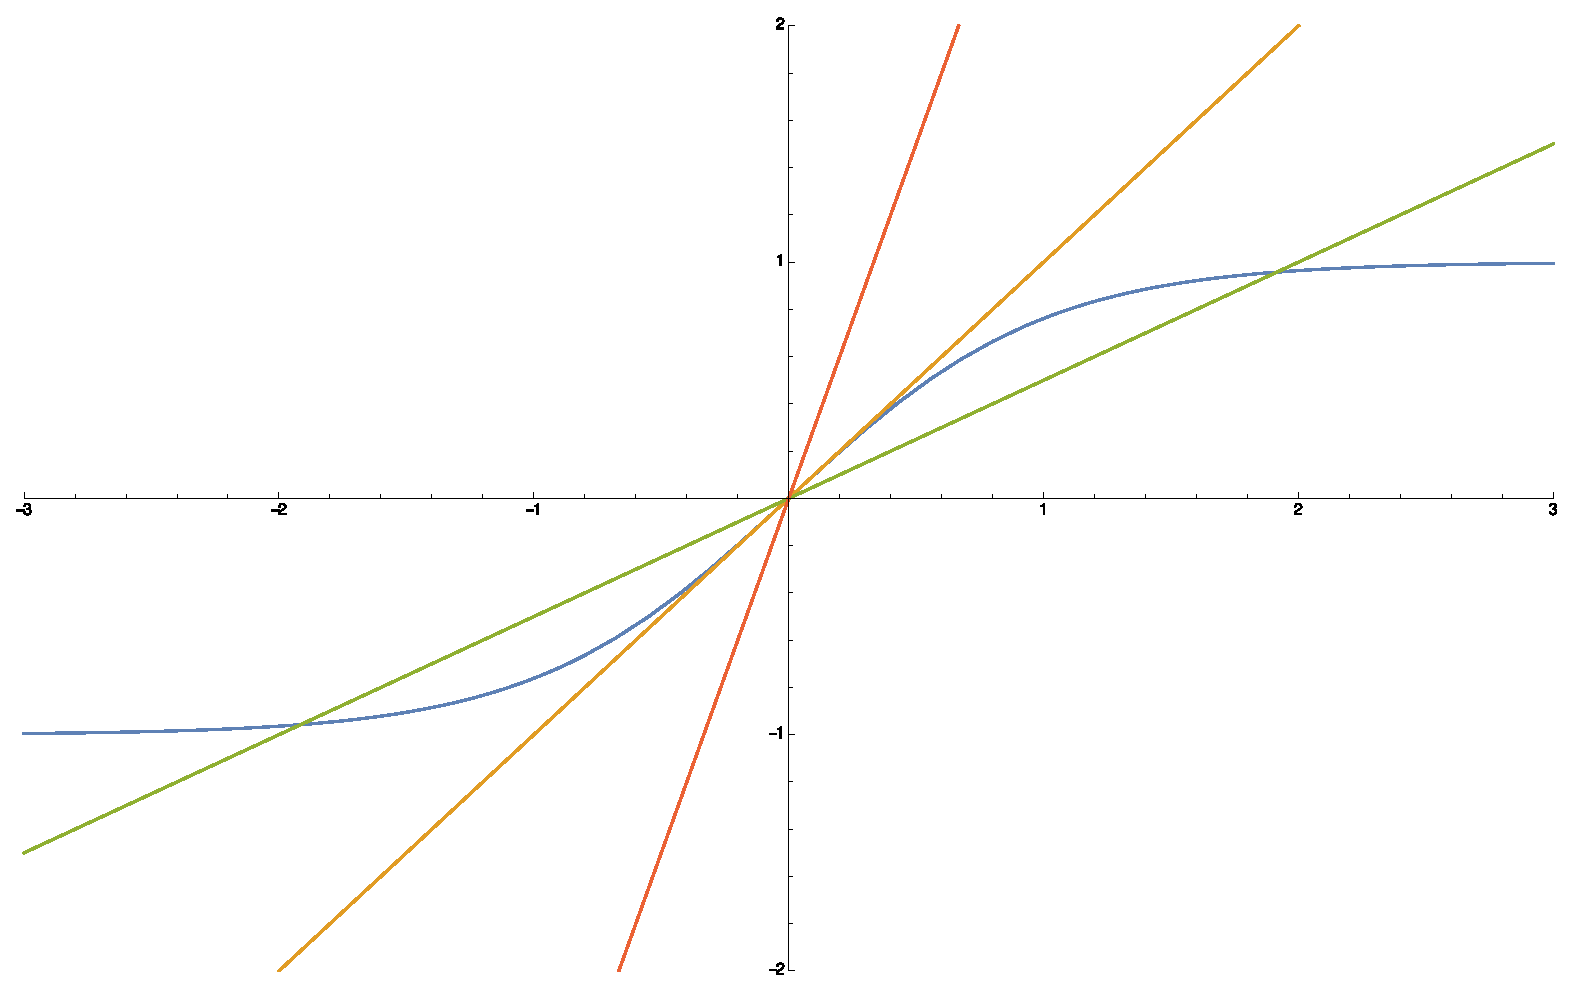
\includegraphics[width=0.65\columnwidth]{tanhpic.eps}
\end{figure}


\noindent
Функция $\tanh x$ ведет себя вблизи нуля линейно: $\tanh x\sim x$.
Из-за симметрии уравнения относительно замены $m\mapsto-m$, всегда
будут иметься как положительные, так и отрицательные решения, поэтому
следить мы будем только за положительными. Из этого и из картинки
можно сделать следующие выводы:
\begin{itemize}
	\item при $T=1$, прямая касается графика $\tanh\tilde{m}$. Это и есть
	искомая критическая точка $T_{c}=1$.
	\item при $T>1$, прямая идет более круто и точек пересечения нет; единственное
	решение уравнения - тривиальное.
	\item при $T<1$, прямая идет полого, и имеются точки пересечения обоих
	графиков, отличные от $m=0$; это и есть наши нетривиальные решения.
	\item при $T\to0$, прямая идет практически горизонтально. Ордината точки
	пересечения стремится к $1$, поэтому решение уравнения $m(T\to0)\to1$.
\end{itemize}
Перейдем обратно от переменной $\tilde{m}$ к переменной $m$ и найдем
асимптотику аналитически. 


\paragraph{Окрестность критической точки $1-T\ll1$}

Вблизи критической точки, $m(T)\ll1$; это позволяет нам разложить
$\tanh(m/T)$ по малости своего аргумента, и переписать уравнение
приближенно как:
\[
m\approx\frac{m}{T}-\frac{1}{3}\left(\frac{m}{T}\right)^{3}\Rightarrow m(T)\approx\sqrt{3(1-T)}
\]

\noindent
В последнем равенстве мы выбросили $T^{2}\approx1$, поскольку мы
интересуемся ведущим порядком разложения по $1-T$. Кроме того, видно,
что наше предположение $m(T)\ll1$ действительно выполняется.


\paragraph{Окрестность нуля $T\ll1$}

Тут видно, что $m(T)\approx1$ (то есть $1-m(T)\ll1$). В таком случае удобно искать решение в виде:
\[
m=1-\varepsilon
\]

\noindent
Здесь $\varepsilon\ll1$. Подставляя, получаем:
$$
1-\varepsilon=\tanh\frac{1-\varepsilon}{T}\approx1-2e^{-2/T}
$$
Таким образом, мы получили поправку к 1: $m\approx1-2e^{-2/T}$.

\begin{figure}[h]
	\caption{Точное решение и найденные асимптотики}
	\centering
	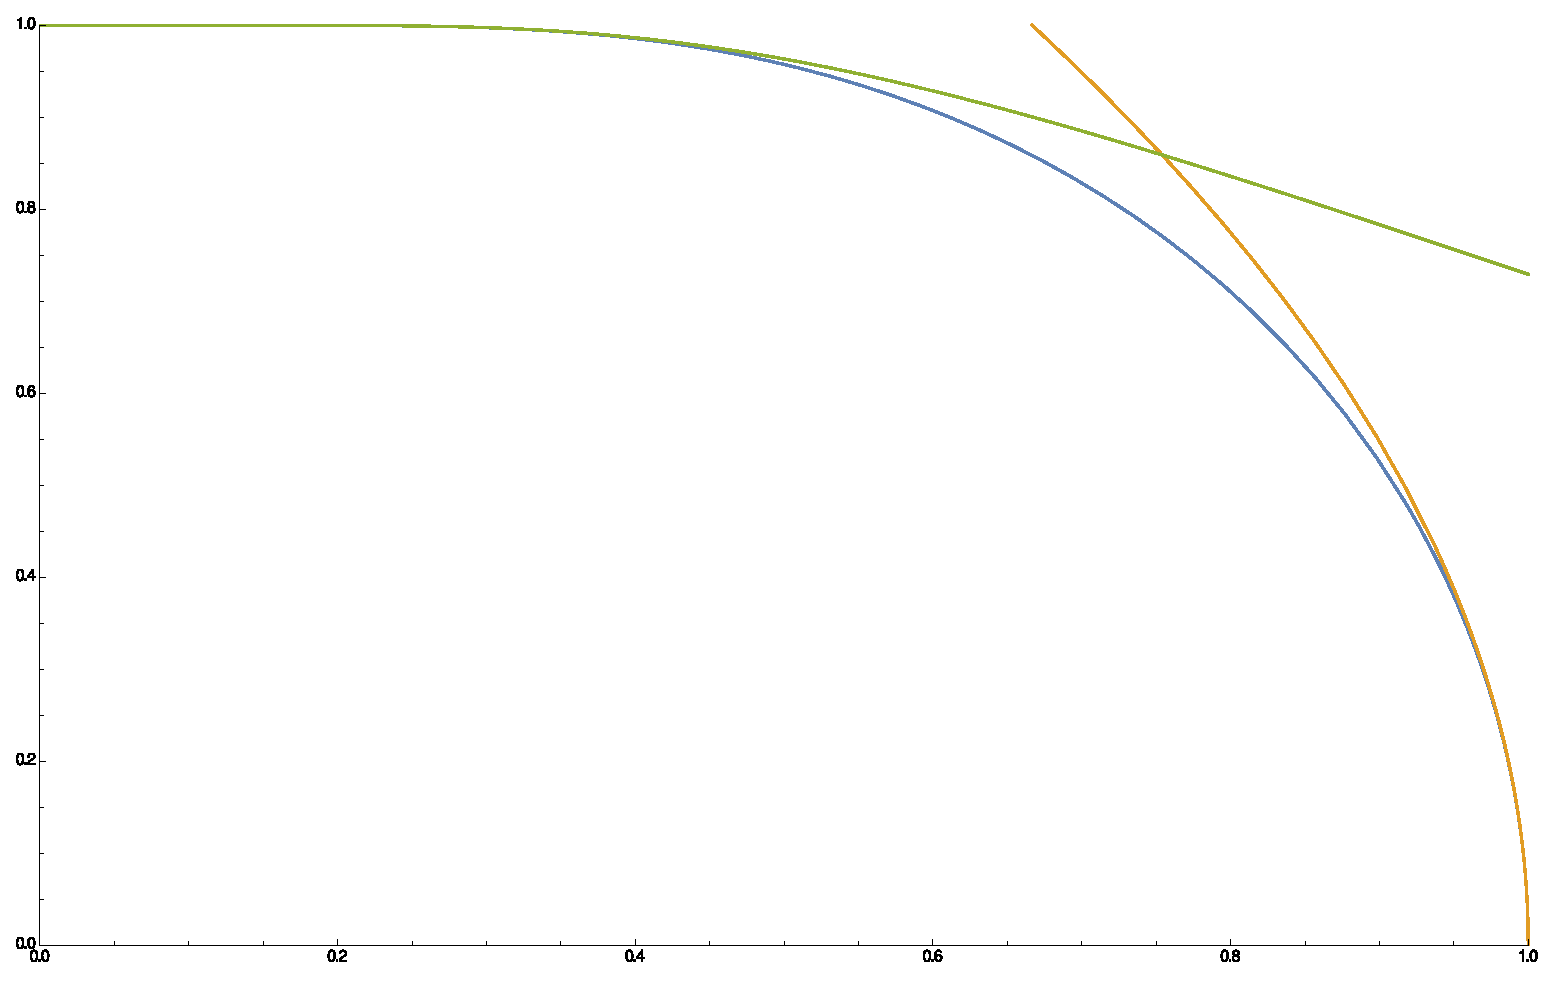
\includegraphics[width=0.65\columnwidth]{plotmagn.eps}
\end{figure}



\subsection{Задача 2 (уровни энергии прямоугольной квантовой ямы)}

Решим уравнение
\[
\tan Ax=\frac{1}{x}
\]

\noindent
при $A\gg1$. Его решения нумеруются целым числом $n$; найти асимптотическое
поведение решений при $n\ll A$ и $n\gg A$.


\subsubsection{Решение}

Будем решать уравнение опять графически. Нарисуем левую и правую часть
уравнения.

\begin{figure}[h]
	\caption{$\tan Ax=\frac{1}{x}$, $A=10$}
	\centering
	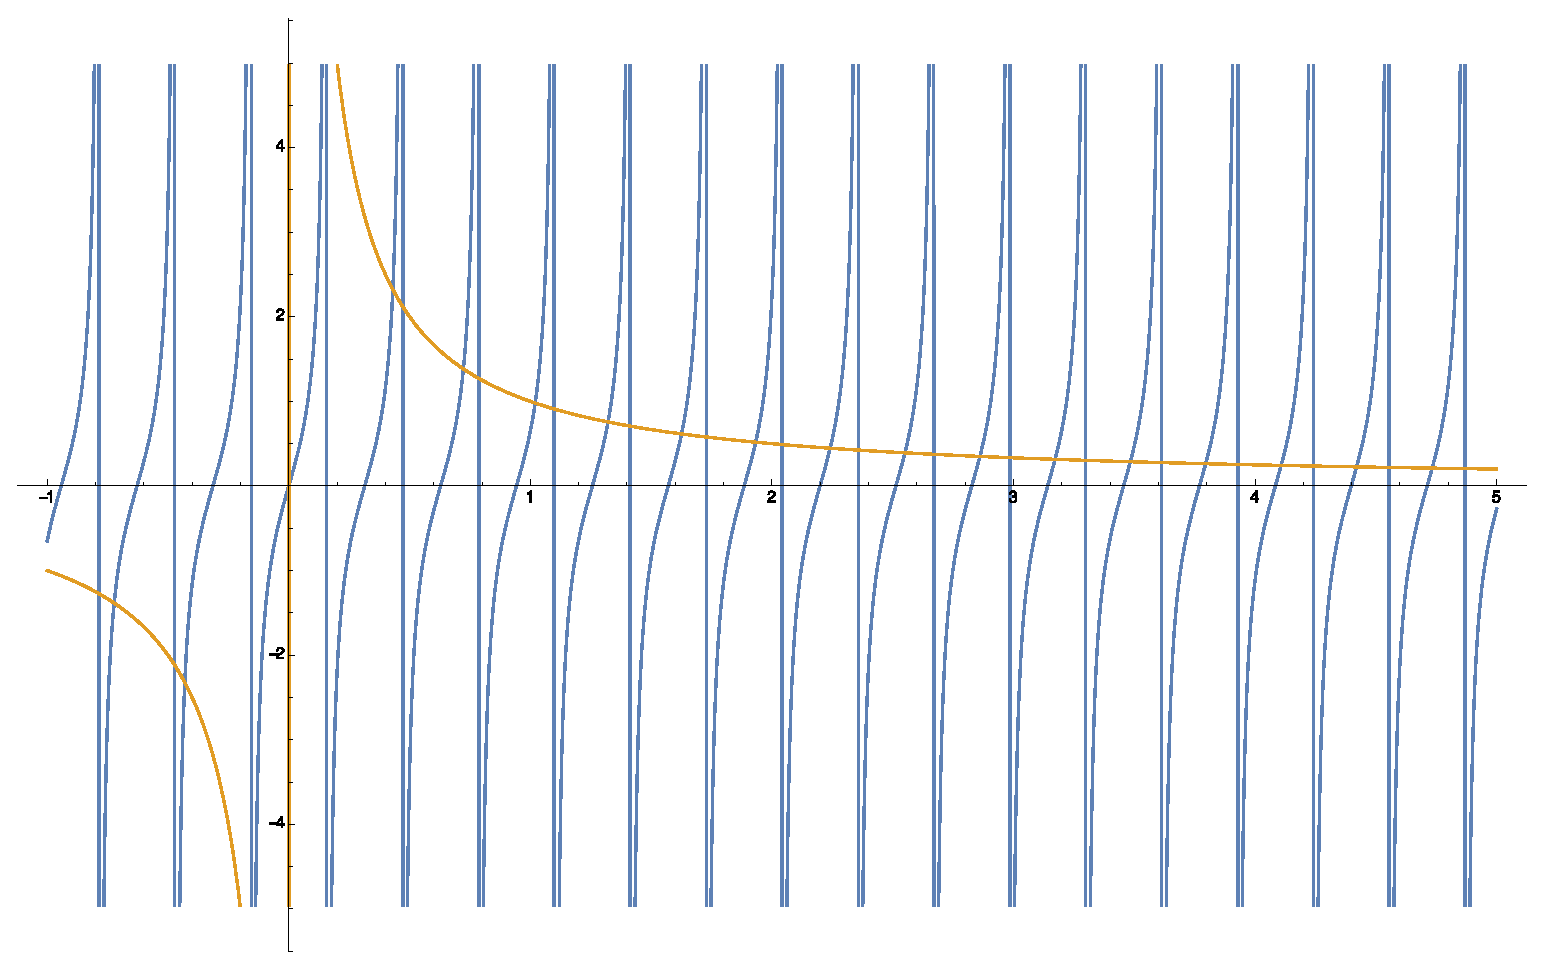
\includegraphics[width=0.65\columnwidth]{plottan.eps}
\end{figure}

\noindent
Видно, что имеется целая серия точек пересечения, которые являются
решением нашего уравнения. Из картинки также можно сделать вывод о
том, вблизи каких точек расположены корни в обоих случаях и в окрестности
каких точек стоит искать решение.


\paragraph{Случай $n\ll A$}

При $n\ll A$, период тангенса мал и все решения лежат вблизи нуля:
$x_{n}\ll1$. Это значит, что в качестве начального приближения можно
заменить правую часть на $+\infty$:
\[
\tan Ax=+\infty\Rightarrow x_{n}^{(0)}\approx\frac{1}{A}\left(\frac{\pi}{2}+\pi n\right)
\]

\noindent
Найдём поправки, используя модификацию метода итераций: метод последовательных
приближений. Введём поправку согласно $x_{n}^{(1)}=\frac{1}{A}\left(\frac{\pi}{2}+\pi n+\epsilon_{n}\right)$
и $|\epsilon_{n}|\ll1$; подстановка в уравнение даёт:

\[
\tan\left(\frac{\pi}{2}+\pi n+\epsilon_{n}\right)=\frac{A}{\frac{\pi}{2}+\pi n+\epsilon_{n}}
\]

\noindent
Разложимся до наинизшего порядка. Левая часть равна $-\frac{1}{\tan\epsilon_{n}}\approx-\frac{1}{\epsilon_{n}}$;
в правой же части в ведущем приближении поправку можно просто выбросить.

\[
\epsilon_{n}\approx-\frac{1}{A}\left(\frac{\pi}{2}+\pi n\right)
\]

\noindent
(видно, что $|\epsilon_{n}|\ll1$, и наше предположение было верным).
Таким образом, в этом случае приближенно ответ записывается как:

\[
x_{n}\approx\frac{1}{A}\left(\frac{\pi}{2}+\pi n\right)-\frac{1}{A^{2}}\left(\frac{\pi}{2}+\pi n\right)
\]



\paragraph{Случай $n\gg A$}

В этом случае $x_{n}\gg1$ и в качестве нулевого приближения можно
заменить правую часть на ноль: 
\[
\tan Ax=0\Rightarrow x_{n}^{(0)}\approx\frac{\pi n}{A}
\]

\noindent
Опять воспользуемся методом последовательных приближений - сделаем
подстановку $x_{n}^{(1)}=\frac{1}{A}(\pi n+\epsilon_{n})$ и $|\epsilon_{n}|\ll1$:

\[
\tan\left(\epsilon_{n}+\pi n\right)=\frac{A}{\epsilon_{n}+\pi n}
\]

\noindent
Проводя разложение левой части $\tan(\pi n+\epsilon_{n})\approx\epsilon_{n}$
и выбрасывая $\epsilon_{n}$ в правой части, мы получаем:

\[
\epsilon_{n}\approx\frac{A}{\pi n}
\]

\noindent
(предположение $\epsilon_{n}\ll1$ тем самым выполнено). Поэтому ответ
записывается как:
\[
x_{n}\approx\frac{\pi n}{A}+\frac{1}{\pi n}
\]

\subsection{Метод итераций}

Один из способов решения трансцедентных уравнений вида $x=f(x)$ есть
метод простых итераций. Сам метод заключается в следующем:
\begin{itemize}
	\item Выберем начальное приближение $x_{0}$
	\item Построим последовательность $\{x_{k}\}$ согласно $x_{k+1}=f(x_{k})$
	\item Если при этом $x_{k}\underset{k\to\infty}{\to}\widetilde{x}$, то
	$\widetilde{x}$ является решением нужного уравнения.
\end{itemize}
Этот метод очень часто применяется для нахождения численных решений;
однако, в случае наличия в задаче большого или малого параметра, он
может помочь найти и приближенный аналитический вид этого решения.
В таком случае, как правило, достаточно заменить последний критерий
на условие $\left|x_{k+1}-x_{k}\right|\ll x_{k}$; при выполнении
этого условия, $x_{k}$ может являться хорошим аналитическим приближением
к ответу. Обычно для того, чтобы увидеть, что либо условие на каком-то шаге выполнилось, либо последовательность приближений расходится, достаточно проделать несколько итераций.


\subsection{Задача 3 (логарифмическая точность)}

При $\alpha\gg 1$ решим уравнение 
\[
x=e^{-\alpha x}
\]

\subsubsection{Решение}

\noindent
Графический анализ показывает, что решение $x\ll1$.

\begin{figure}[h]
	\caption{$x=e^{-\alpha x}$, $\alpha=20$}
	\centering
	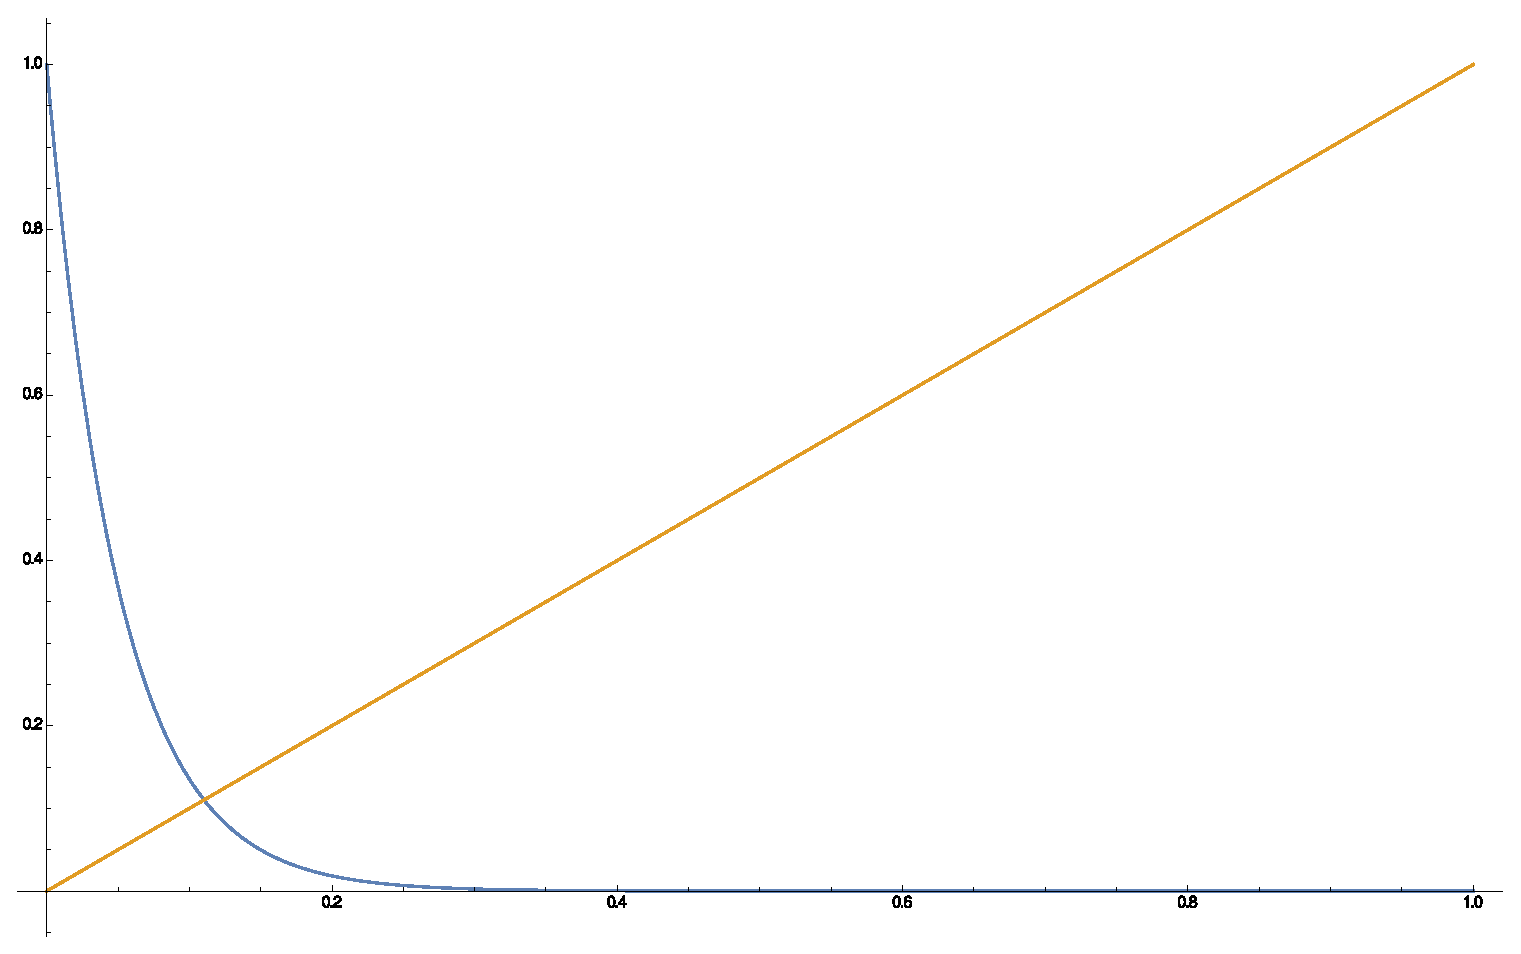
\includegraphics[width=0.65\columnwidth]{plotexp.eps}
\end{figure}

\noindent
Кроме того, видно,
что $\alpha x$ не может быть малым числом: в противном случае $e^{-\alpha x}\approx1\Rightarrow x\approx1$,
что противоречит этому анализу. Для решения мы воспользуемся методом
итераций, но применим его не к исходному уравнению, а к переписанному
в виде $x=\frac{1}{\alpha}\ln\frac{1}{x}$. 
\begin{itemize}
	\item В качестве начального приближения давайте возьмём произвольное число
	$x_{0}\sim1$. В дальнейшем мы увидим, что от него зависеть ничего
	не будет.
	\item Первое приближение даёт $x_{1}=\frac{1}{\alpha}\ln\frac{1}{x_{0}}$.
	Поскольку $x_{1}\ll x_{0}$, то $\left|x_{0}-x_{1}\right|\approx x_{0}$
	и это приближение не является хорошим.
	\item Второе приближение даёт $x_{2}=\frac{\ln\alpha}{\alpha}-\frac{1}{\alpha}\ln\ln\frac{1}{x_{0}}$.
	В силу $\alpha\gg1$, второе слагаемое мало и его можно выбросить
	(и тем самым выпадает зависимость от начального приближения). В таком
	случае $x_{2}\gg x_{1}$ и приближение опять-таки не является хорошим.
	\item Третье приближение даёт $x_{3}=\frac{\ln\alpha}{\alpha}-\frac{\ln\ln\alpha}{\alpha}$.
	В этом случае поправка действительно оказывается малой: $\left|x_{3}-x_{2}\right|=\frac{\ln\ln\alpha}{\alpha}\ll x_{2}=\frac{\ln\alpha}{\alpha}$;
	это наконец и означает, что мы нашли хорошее приближение, а также
	ведущую поправку к нему.
\end{itemize}
Таким образом, ответ приближенно записывается как $x\approx\frac{\ln\alpha}{\alpha}$.

\begin{figure}[h]
	\caption{Численное решение $x=e^{-\alpha x}$ и его асимптотика}
	\centering
	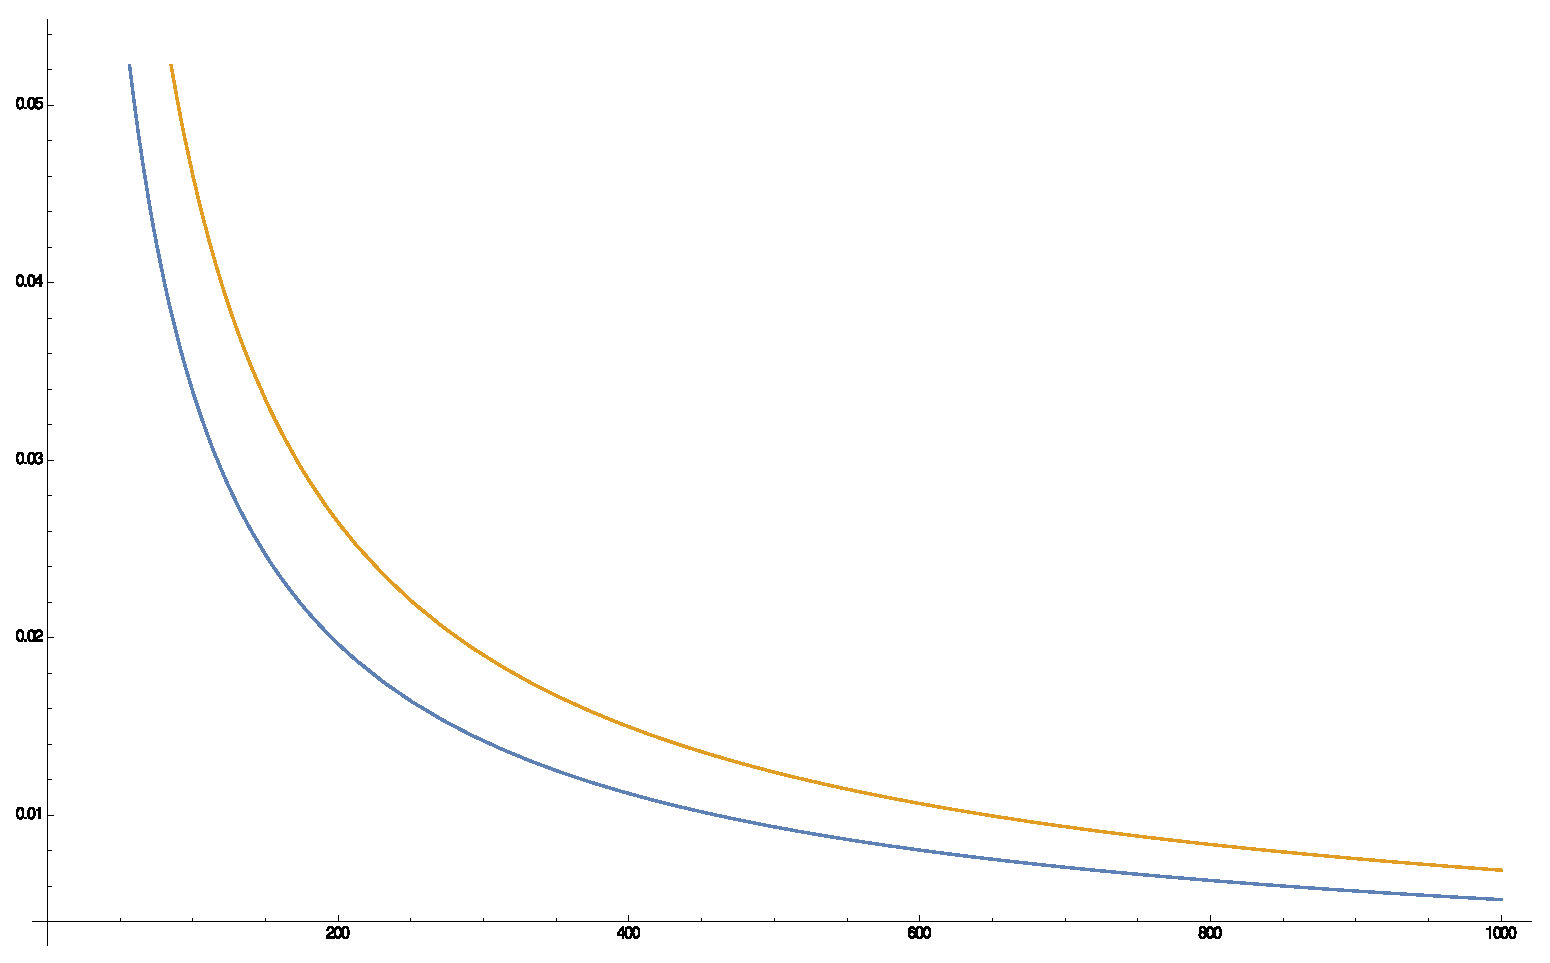
\includegraphics[width=0.65\columnwidth]{plotexpsol.eps}
\end{figure}

Из-за того, что логарифм - медленно растущая функция, первое приближение работает в данном интервале не очень хорошо. Более точным будет учесть поправку: 
\begin{figure}[h]
	\caption{Численное решение $x=e^{-\alpha x}$ и его асимптотика с учётом первой поправки}
	\centering
	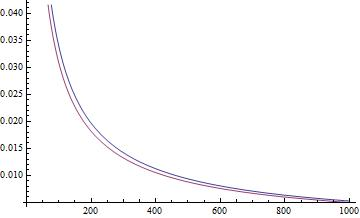
\includegraphics[width=0.65\columnwidth]{product_log.jpg}
\end{figure}

\newpage

\subsection{Задачи для домашнего решения}

\noindent \textbf{Упражнение 1}

\noindent При $\alpha\gg 1$ и $\alpha\ll 1$ приближенно решите уравнениe

\noindent 
\begin{align*}
x & =1+\exp(-\alpha x).
\end{align*}

\vspace{15pt}
\noindent \textbf{Упражнение 2}

\noindent При $\alpha\gg 1$ и $\alpha\ll 1$ приближенно решите уравнениe

\noindent 
\begin{align*}
\ln x & =e^{-\alpha x}.
\end{align*}

\vspace{15pt}
\noindent \textbf{Упражнение 3}

\noindent На семинаре была определена функция Ламберта $x(\lambda)$, которая при $\lambda\geq 0$ задается как решение уравнения

\noindent 
\begin{align*}
xe^{x} & =\lambda.
\end{align*}

\noindent При $-\frac{1}{e}<\lambda<$0 это уравнение имеет два решения: $x_{1}(\lambda)>-1$ и $x_{2}(\lambda)<-1$ (для непрерывности обычно именно $x_{1}(\lambda)$ называют функцией Ламберта на $-\frac{1}{e}\leq\lambda<0$). При $\lambda=-\frac{1}{e}$, как легко увидеть, $ x_{1}=x_{2}=-1$, а при $\lambda<-\frac{1}{e}$ действительных решений нет. Приближенно найдите $x_{1}(\lambda)$, $x_{2}(\lambda)$ при $\lambda<0$, $|\lambda|\ll 1$. 

\vspace{15pt}
\noindent \textbf{Упражнение 4}

\noindent Найдите $x_{1}(\lambda)$, $x_{2}(\lambda)$ из упражнения 3 при $\lambda>-\frac{1}{e}$, $|\lambda+\frac{1}{e}|\ll 1$. \\\\

\vspace{15pt}
\noindent \textbf{Задача 1}

\noindent Приближенно решите уравнение

\noindent 
\begin{align*}
\tanh\alpha x & =\arctan x
\end{align*}

\noindent при $0<\alpha-1\ll 1$ и при $\alpha\gg1$.

\vspace{15pt}
\noindent \textbf{Задача 2}

\noindent При $\alpha\ll 1$ положительные решения неравенества

\noindent 
\begin{align*}
\left|\cos x+\alpha\frac{\sin x}{x}\right| & >1
\end{align*}

\noindent разбиваются на серию зон, нумеруемых целыми числами $k=0,1,...$ Определить ширину $k$-ой зоны при $k\gg1$.
\end{document}
